\documentclass[a4paper,12pt]{article}
\usepackage[utf8]{inputenc}
\usepackage[T1]{fontenc}
\usepackage[ngerman]{babel}
\usepackage{graphicx}
\usepackage{geometry}
\usepackage{setspace}
\usepackage{float}
\usepackage{hyperref}
\usepackage{tabularx}
\usepackage{booktabs}
\usepackage{cite}
\usepackage{array}
\usepackage{longtable}
\graphicspath{ {./assets/} }
\geometry{a4paper, left=2cm, right=2cm, top=2cm, bottom=2cm}
\onehalfspacing

\setlength{\parindent}{0pt}

\usepackage{helvet}
\renewcommand\familydefault{\sfdefault}

\newcommand{\autor}{Elyssa Jane Dean}
\newcommand{\geburtsdatum}{27.09.1992}
\newcommand{\arbeitgeber}{IUSCare GmbH Ambulante Intensivpflege}
\newcommand{\kursbezeichnung}{Basiskurs FAI: Fachkraft für außerklinische Intensivpflege}
\newcommand{\kurszeitraum}{27.01.2025 - 04.02.2025}
\newcommand{\abgabedatum}{\today}

\title{\textbf{Facharbeit}}
\author{
    \autor \\
    Geburtsdatum: \geburtsdatum \\
    Arbeitgeber: \arbeitgeber \\
    Kursbezeichnung: \kursbezeichnung \\
    Zeitraum des Kurses: \kurszeitraum \\
    Abgabedatum: \abgabedatum
}
\date{}

\begin{document}

\begin{titlepage}
	\centering
	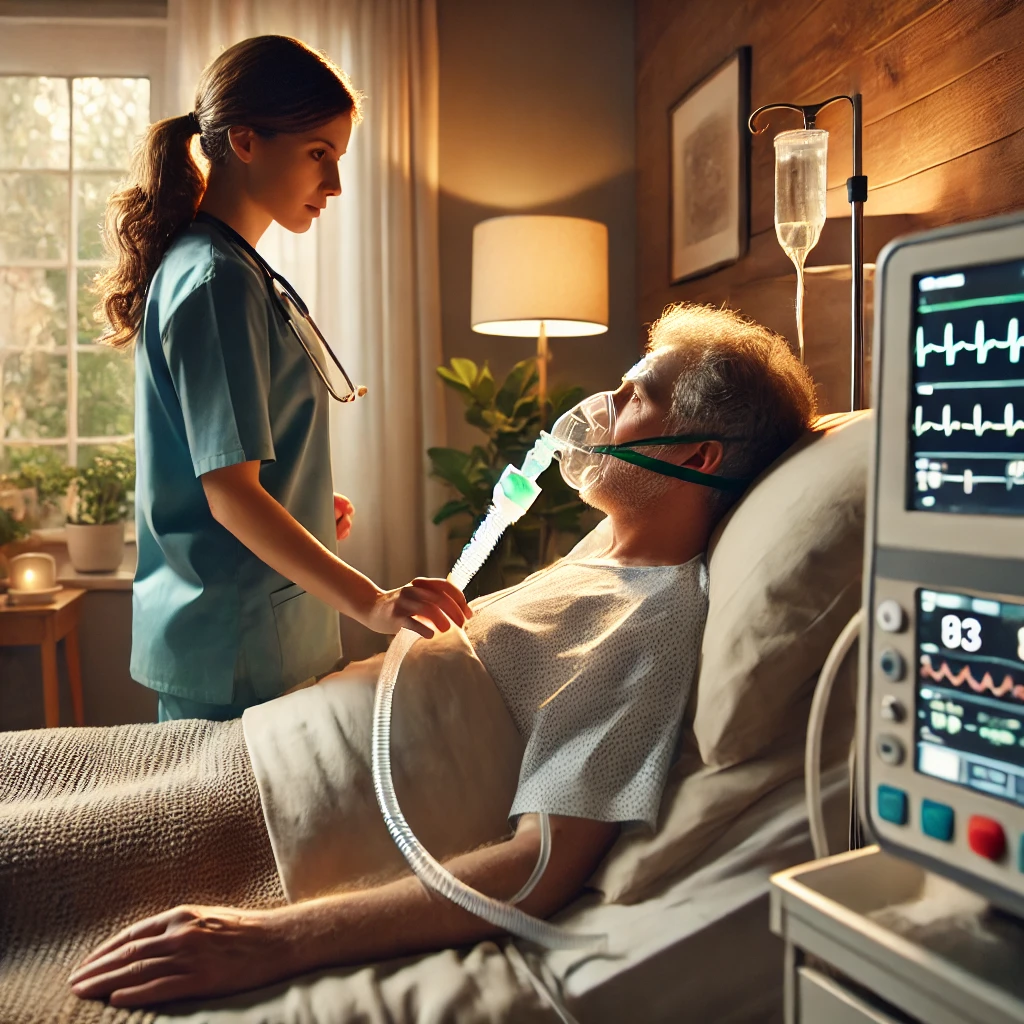
\includegraphics[width=\textwidth]{banner}
	\vspace{0.5cm}
	{\large \textbf{\kursbezeichnung} \par}
	\vspace{0.5cm}
	{\large \textbf{\autor} \par}
	\vspace{0.5cm}
	{\large Geburtsdatum: \geburtsdatum \par}
	\vspace{0.5cm}
	{\large Arbeitgeber: \arbeitgeber \par}
	\vspace{0.5cm}
	{\large Zeitraum des Kurses: \kurszeitraum \par}
	\vspace{0.5cm}
	{\large Abgabedatum: \abgabedatum \par}
\end{titlepage}

\tableofcontents
\newpage

\section{Einleitung}
Ich bin \autor. Ich habe meinen insgesamt fünfjährigen
Bachelorabschluss in Nursing auf den Philippinen im Jahr 2012 abgeschlossen
und meine Anerkennung als Gesundheits- und Krankenpflegerin (GKP) in
Deutschland im März 2024 erhalten.
Ich habe dreieinhalb Jahre in Vollzeit in einer orthopädischen Klinik in
Braunfels gearbeitet, bevor ich im Oktober 2024 zur Konstant Ambulanten
Intensivpflege gewechselt bin, die nun als IUSCare GmbH Ambulante Intensivpflege bekannt ist.
Zusätzlich habe ich zwei Jahre in den Philippinen in der medizinischen und
chirurgischen Abteilung gearbeitet und anschließend drei Jahre im OP-Complex.
Diese Abteilung umfasst den Operationssaal, den Aufwachraum, die Endoskopie
und den Entbindungssaal.
Ich habe mich entschieden, in die ambulante Intensivpflege zu wechseln, da ich
das Bedürfnis hatte, eigenständiger zu arbeiten und Neues zu lernen. Mein
Wissen über das Thema „Beatmung“ war begrenzt, weshalb ich mich intensiver
damit beschäftigen wollte.

\section{Biografie und Vorstellung des Patienten}
Mein Patient ist männlich, 82 Jahre alt, wurde am 14.12.1942 geboren
und hat Pflegegrad 4. Er ist verwitwet und
lebt derzeit mit seiner Lebensgefährtin zusammen.
In seiner Freizeit spielt er gerne Englisch Horn
und war Mitglied einer Kurverwaltung in Bad Orb.
Im Juni 2015 wurde bei ihm ein Tonsillenkarzinom links diagnostiziert. Im
August 2015 erfolgte eine Tonsillektomie links mit anschließender primärer
Radiochemotherapie im Klinikum Schwalmstadt in Marburg.
Am 15.06.2024 wurde eine Hypopharynx-Tamponade sowie ein plastisches
Tracheostoma mit operativer Ligatur der A. carotis externa rechts angelegt.
Vom 24.06.2024 bis zum 08.08.2024 befand sich der Patient in den
Asklepios-Schwalm-Eder-Kliniken aufgrund einer respiratorischen
Globalinsuffizienz mit Azidose und CO$_2$-Narkose infolge einer
Sekretverlegung im Tracheostoma. Dies führte zu einem beginnenden septischen
Schock. Während dieses Aufenthalts wurde er am 26.06.2024 und 08.07.2024 mit
einer BiPAP-Beatmung oder Beatmung auf zwei Druckniveaus mit Druckunterstützung beatmet.
Am 02.07.2024 wurde eine PEG-Sonde angelegt, da er unter Schluckstörungen leidet.

\section{Grunderkrankung: Mandelkrebs}

\subsection{Definition}
Mandelkrebs, auch als Tonsillenkarzinom bezeichnet, ist eine bösartige
Erkrankung der Gaumenmandeln. Sie gehört zur Gruppe der Mund-Rachen-Tumoren
(Oropharynxkarzinome) \cite{germanyMandelkrebsSpezialistenInformationen}.
Männer sind dreimal häufiger betroffen als Frauen.
Das größte Risiko für die maligne Entstehung besteht bei regelmäßigem oder
exzessivem Konsum von Tabak und Alkohol. Zudem stellt eine Infektion mit
Humanen Papillomviren einen wesentlichen Risikofaktor dar \cite{doccheckTonsillenkarzinom}.

\subsection{Merkmale der Grunderkrankung}
Da es keine spezifischen Vorstadien gibt, ist Mandelkrebs oft schwer frühzeitig
zu erkennen. Zu den unspezifischen Symptomen gehören Schluckbeschwerden,
Schwellungen im Halsbereich, anhaltende Heiserkeit, Husten, Mundgeruch sowie
Probleme beim Essen und Trinken \cite{germanyMandelkrebsSpezialistenInformationen}.

\subsection{Diagnose}
Zur Feststellung einer Diagnose können verschiedene Untersuchungen durchgeführt
werden. Dazu gehören die Spiegeluntersuchung, die Panendoskopie, die Biopsie,
die Sonographie, die Computertomographie, die Magnetresonanztomographie sowie
die Szintigraphie des Rachenraumes. Der Tumor wird anschließend klassifiziert,
unter Berücksichtigung von Metastasen in benachbarten Organen, um eine geeignete
Therapie festzulegen. Die Stadieneinteilung des Mandelkrebses unterscheidet sich
nicht wesentlich von der allgemeinen T-Klassifikation der Tumoren. Je nach Größe
oder Ausdehnung des Tumors gibt es folgende Stadien: Im T1-Stadium ist der Tumor
kleiner als 2 cm, im T2-Stadium hat der Tumor eine Größe von 2 bis 4 cm. Das T3-Stadium
beschreibt einen Tumor, der größer als 4 cm ist. Im T4-Stadium hat der Tumor
unabhängig von der Größe umliegende Gewebestrukturen infiltriert. Am häufigsten
sind hiervon der Hals, die Wangen und die Zungengrundmuskulatur betroffen \cite{germanyMandelkrebsSpezialistenInformationen}.

\subsection{Medikamentöse Therapie}

Der Patient hat aktuell folgende Medikamente nach AAO vom 8.8.2024.

\begin{longtable}{|p{4cm}|p{2cm}|p{2cm}|p{3cm}|p{5cm}|}
	\hline
	\textbf{Wirkstoff}     & \textbf{Stärke} & \textbf{Form} & \textbf{Täglich} & \textbf{Hinweise}      \\
	\hline
	Insulin lispro         & 100 E           & Lösung        & nach Schema      & Blutzuckersenkung      \\
	\hline
	Melperon               & 25 mg           & Tabl          & 0-0-1            & Antipsychotika         \\
	\hline
	Torasemid              & 10 mg           & Tabl          & 1-0-0            & Diuretika              \\
	\hline
	Salbutamol             & 5 mg            & LOV           & nach Bedarf      & Schleimlösung          \\
	\hline
	Ipratropium Kation     & 0.25 mg         & LOV           & nach Bedarf      & Schleimlösung          \\
	\hline
	Insulin lispro isophan & 25/75           & Susp          & 30 IE            & Blutzuckersenkung      \\
	\hline
	Acetylsalicylsäure     & 100 mg          & Tabl          & 1-0-0            & Blutverdünnung         \\
	\hline
	Atorvastatin           & 20 mg           & Tabl          & 1-0-0            & Blutfettwertereduktion \\
	\hline
	Escitalopram           & 10 mg           & Tabl          & 1-0-0            & Magenschutz            \\
	\hline
	Mirtazapin             & 15 mg           & Tabl          & 0-0-1            & Depressive Erkankungen \\
	\hline
	Jardiance              & 10 mg           & Tabl          & 1-0-0            & Blutzuckersenkung      \\
	\hline
\end{longtable}

\newpage

Der Patient erhält folgende Bedarfsmedikamente.

\begin{longtable}{|p{4cm}|p{2cm}|p{2cm}|p{3cm}|p{5cm}|}
	\hline
	\textbf{Wirkstoff} & \textbf{Stärke} & \textbf{Form}  & \textbf{Täglich}                        & \textbf{Hinweise} \\
	\hline
	Piritramid         & 7.5 mg          & Ampulle        & 1/2 amp s.c.                            & Schmerztherapie   \\
	\hline
	Movicol            & -               & Beutel         & bis max. 3x1                            & Abführmittel      \\
	\hline
	Zopiclon           & 7.5 mg          & Halbe Tablette & 0-0-0-1, möglichst ausschleichen        & Einschlafhilfe    \\
	\hline
	Lorazepam          & 1 mg            & Tablette       & 1/2 Tbl über PEG, max. 3x je 24 Stunden & Beruhigungsmittel \\
	\hline
\end{longtable}

Der Patient erhält eine PEG-Sonde mit folgendem Inhalt.

\begin{longtable}{|p{4cm}|p{2cm}|p{3cm}|p{5cm}|}
	\hline
	\textbf{Wirkstoff}                    & \textbf{Form} & \textbf{Täglich}                      & \textbf{Hinweise}       \\
	\hline
	Nutricomp Energy HP Fibre             & Flasche       & 1-1-0, läuft 170ml/h                  & Ernährungsunterstützung \\
	\hline
	Nutricomp Standard mit Ballaststoffen & Flasche       & läuft 170ml/h                         & Ernährungsunterstützung \\
	\hline
	H2O Wasser + Tee                      & Flüssigkeit   & 1-0-1, über PEG, solange 2 Mahlzeiten & Flüssigkeitszufuhr      \\
	\hline
\end{longtable}

\subsection{Verlauf}
In den meisten Fällen wurde der Tumor mit einem großen Sicherheitsabstand chirurgisch
entfernt. Nach der Operation folgte in einigen Fällen eine Radiotherapie, Chemotherapie
oder eine kombinierte Radiochemotherapie. Die Prognose hängt sehr stark vom Stadium
der Diagnose ab, und Metastasen beeinflussen den Krankheitsverlauf negativ. So ergibt
sich für den Mandelkrebs eine 5-Jahres-Überlebensrate, die je nach Stadium unterschiedlich
ist. Im T1-Stadium leben etwa 80–90\% der Patienten noch fünf Jahre nach der Diagnose,
im T2-Stadium sind es ca. 70–75\%, im T3-Stadium liegt die Überlebensrate bei etwa
40–50\%, und im T4-Stadium beträgt sie nur noch ca. 10–35\% \cite{germanyMandelkrebsSpezialistenInformationen}.

\subsection{Nebendiagnose}

Neben der Grunderkrankung bestehen mehrere Nebendiagnosen. Der Patient
leidet unter einer Epiglottitis DD mit begleitender bronchopulmonaler
Infektion, die fortlaufende Infektionen in den Bronchiolen zur Folge hat.
Diese können zu Diffusions- oder Perfusionsproblemen beim Gasaustausch führen,
was eine maschinelle Beatmung erforderlich machen kann. Zusätzlich liegt eine
Diabetes mellitus Typ 2 vor, die mit einer intensivierten Insulintherapie
sowie oralen Antidiabetika behandelt wird.
Des Weiteren besteht ein rechtsfrontaler Hirninfarkt ischämischer Genese.
Falls es in diesem Zusammenhang zu einer Beeinträchtigung der Atmung kommt,
muss eine künstliche Beatmung erfolgen. Zusätzlich wurde eine schwere
depressive Episode im Rahmen einer Anpassungsstörung diagnostiziert,
die sich auf die Alarmgrenzen der Beatmungsparameter auswirken kann.
Er leidet außerdem unter arterieller Hypertonie, die im Falle einer
unzureichenden Einstellung Auswirkungen auf die Beatmung haben kann.
Eine chronische Niereninsuffizienz im Stadium 3, vermutlich aufgrund
einer diabetischen Nephropathie, ist ebenfalls vorhanden.
Im Rahmen einer akuten Nierenschädigung kann es zu einer zunehmenden Schädigung
und Funktionseinschränkung der Lunge kommen \cite{IntensivmedizinWieNieren}.
Durch entsprechende vorsichtige Flüssigkeitsbilanzierung mit harntreibenden Medikamenten
oder einer Dialyse können diese Komplikationen vorgebeugt werden.
Zusätzlich leidet der Patient unter einer Hämochromatose, die in der
Vergangenheit mit Aderlässen behandelt wurde. Die letzte Therapie wurde
bei einem Ferritinwert unter 50 beendet. Falls diese Erkrankung nicht beachtet
wird, kann sie zu Perfusionsproblemen beim Gasaustausch führen. Darüber hinaus
besteht eine benigne Prostatahyperplasie, die jedoch keinen Einfluss auf die
Beatmung hat. Ebenso hat der Patient eine Neurodermitis, die sich nicht auf
seine respiratorische Situation auswirkt.

\section{Beatmungsformen}

\subsection{PSV - Pressure Support Ventilation}

Die druckunterstützte Beatmungsform PSV (Pressure Support Ventilation), auch als
ASB-Beatmung (Assisted Spontaneous Breathing) bekannt, dient dazu, die
Eigenatmung des Patienten zu unterstützen. Sie wird häufig in Kombination mit
der CPAP-Beatmung eingesetzt \cite{PSVASBDruckunterstuetzte}.
Dabei wird der vom Patienten initiierte Atemzug
durch einen zusätzlichen Druck der Beatmungsmaschine verstärkt.
Voraussetzung für diese Beatmungsform ist eine erhaltene Eigenatmung mit
intakter Atemmuskulatur und funktionierendem Atemantrieb, wenngleich die
Atemmuskulatur geschwächt sein kann \cite{PSVBeatmungDruckunterstuetzteBeatmung}.
Die wichtigsten Beatmungsparameter der PSV-Beatmung sind der positive
endexspiratorische Druck (PEEP), der am Ende der Ausatmung aufrechterhalten
wird, sowie die Druckunterstützung bei jedem spontanen Atemzug, die als
Pressure Support (PS) oder $\Delta$pASB bezeichnet wird. Die Inspirations- und
Exspirationszeiten können ebenfalls eingestellt werden, wobei der inspiratorische
Trigger bestimmt, mit welcher Sensibilität das Beatmungsgerät auf die Einatemversuche
des Patienten reagiert. Der exspiratorische Trigger erfasst den Beginn der Ausatmung.
Zudem kann die sogenannte Rampe, also die Geschwindigkeit, mit der der Druck zu Beginn
der Inspiration ansteigt, individuell angepasst werden \cite{PSVASBDruckunterstuetzte}.

\subsection{PCV - Pressure Controlled Ventilation}

Die druckkontrollierte Beatmung (PCV, Pressure Controlled Ventilation) stellt
eine Beatmungsform dar, bei der die Maschine die Steuerung der Atmung vollständig
übernimmt. Im Gegensatz zur PSV ist hier keine Spontanatmung erforderlich.
Diese Form der Beatmung wird insbesondere bei Patienten mit schwacher
Atemmuskulatur und fehlendem Atemantrieb angewandt. Dabei wird der
Inspirationsdruck (pInsp) in Millibar definiert und mit einer bestimmten
Atemfrequenz (Freq.) kombiniert.
Weitere relevante Parameter sind der positive endexspiratorische Druck (PEEP)
sowie der maximale Inspirationsdruck (pMax), der sicherstellt, dass ein
vorgegebenes Druckmaximum nicht überschritten wird. Dadurch wird die Lunge
vor einer Überdehnung und den damit einhergehenden Sekundärschäden geschützt.
Das Inspirations-Exspirationsverhältnis (I:E) kann ebenfalls reguliert werden,
um eine optimale Anpassung an die Bedürfnisse des Patienten zu gewährleisten \cite{doccheckDruckkontrollierteBeatmung}.

\subsection{Vergleich zwischen PSV und PCV}

Die PSV-Beatmung unterstützt die Eigenatmung des Patienten, wobei die
Atmung durch den Patienten selbst gesteuert und initiiert wird.
Bei der PCV-Beatmung hingegen übernimmt das Beatmungsgerät die vollständige
Steuerung der Atmung, sodass in der Regel keine eigene Spontanatmung mehr
vorliegt \cite{PSVBeatmungDruckunterstuetzteBeatmung}.
Beide Beatmungsformen haben ihre spezifischen Vorteile. Die PSV-Beatmung
ermöglicht eine effektive Atemunterstützung bei gleichzeitiger Wahrung
eines hohen Komforts für den Patienten \cite{InvasiveUndNichtinvasive}.
Der PCV-Modus bietet wiederum den Vorteil,
dass der Patient während der Exspirationsphase frei ausatmen kann.
Die festgelegte maximale Druckbegrenzung (pMax) gewährleistet zudem
ein hohes Maß an Sicherheit.
Allerdings gibt es auch Risiken. Eine drastische Reduktion der Atemarbeit
des Patienten kann dazu führen, dass der PSV-Modus nicht ausreicht. Daher
muss regelmäßig überprüft werden, ob die gewählte Beatmungsform den
Bedürfnissen des Patienten entspricht. Bei der PCV-Beatmung besteht
die Gefahr einer unbeabsichtigten Hypoventilation oder Hyperventilation.
Zudem können plötzliche intrathorakale Drucksteigerungen, beispielsweise
durch Husten oder Pressen, ein Barotrauma der Lunge verursachen.
Um diese Risiken zu minimieren, müssen enge Alarmgrenzen für das
Tidalvolumen festgelegt und auf eine ausreichende Narkosetiefe geachtet
werden \cite{doccheckDruckkontrollierteBeatmung}.

\subsection{Alarmgrenzen bei der Beatmung}

Die Festlegung der Alarmgrenzen richtet sich in der Regel nach der
ärztlichen Verordnung. Da invasive Beatmungsmodi mit spezifischen Risiken
verbunden sind, ist es die Aufgabe der Pflegefachkraft, die Parameter
kontinuierlich zu überwachen und zu überprüfen, ob sie weiterhin für
den Patienten geeignet sind. Falls eine Anpassung erforderlich ist,
müssen neue Beatmungsparameter ärztlich verordnet werden.
Die Alarmgrenzen dürfen weder zu eng noch zu weit gesetzt werden.
Zu enge Grenzen können dazu führen, dass der Patient durch häufige
Fehlalarme gestört wird. Sind die Alarmgrenzen hingegen zu weit
gefasst, besteht das Risiko, dass Komplikationen zu spät erkannt
werden oder sogar unbemerkt bleiben.

\subsection{Zugang der Beatmung}

Es gibt zwei Hauptarten der Beatmung: die nicht-invasive Beatmung (NIV) und die invasive Beatmung.

\subsubsection{Nicht Invasive Beatmung}

Die nicht-invasive Beatmung (NIV) ist eine Beatmung, bei der keine invasiven Beatmungszugänge
wie ein Endotrachealtubus oder eine Trachealkanüle verwendet werden. Sie stellt eine
Atemtherapie dar, die bei Patienten zum Einsatz kommt, die Schwierigkeiten haben, ausreichend
Sauerstoff aufzunehmen oder Kohlendioxid abzugeben \cite{NichtinvasiveBeatmungUltimative}.
Bei dieser Art der Beatmung werden
verschiedene Maskenarten verwendet, um den Patienten nicht-invasiv zu beatmen. Zu den Maskenarten
zählen Nasenmasken, Nasen-Mundmasken, Gesichtsmasken und Beatmungshelme \cite{schleicherNIVBeatmungWannSetzt2019}.
Die NIV wird in verschiedenen Situationen eingesetzt. Zu den häufigsten Indikationen gehören
Oxygenierungsstörungen wie sie bei Asthma auftreten, Weaning bei Patienten mit chronisch obstruktiver
Lungenerkrankung (COPD), das akute Lungenversagen, kardiales Lungenödem und Rauchgasintoxikation
wie Kohlenmonoxid- oder CO-Vergiftung. Ein weiteres Anwendungsgebiet ist die Behandlung von
exazerbierten chronisch obstruktiven Lungenerkrankungen (COPD) \cite{NichtinvasiveBeatmungUltimative}.
Die Vorteile der NIV liegen in der effektiven Therapie mit einem niedrigen Infektionsrisiko und
verbesserten Überlebensraten. Studien zeigen, dass Patienten mit NIV eine Lebensverlängerung von
drei bis fünf Jahren haben können.
Ein weiterer Vorteil ist die geringe Invasivität, da keine
tiefen Analgosedierungen erforderlich sind. Zudem fällt das Weaning, also die Entwöhnung von der
Beatmung, im Vergleich zur invasiven Therapie leichter. Ein wichtiger Vorteil ist, dass die Kommunikation
mit dem Patienten während der NIV erhalten bleibt und sogar kurze Unterbrechungen für Nahrungsaufnahme
und Mobilisation möglich sind \cite{InvasiveUndNichtinvasive}.
Trotz der vielen Vorteile gibt es auch einige Nachteile bei der NIV. Zu den möglichen Problemen gehören
Konjunktivitis, die durch ausströmende Luft bei einer Leckage der Maske im Bereich der Nasenwurzel
verursacht wird. Zudem bietet die NIV keinen sicheren Aspirationsschutz, was bedeutet, dass es zu
Aspiration und Aerophagie kommen kann. Durch den Einsatz einer Magensonde und Unterstützungsdrücken
unter 25 mBar lässt sich dieses Risiko jedoch weitgehend minimieren. Ein weiteres Problem ist, dass die
Maske sich während der Behandlung verschieben kann, was zu einem unsicheren Atemweg führt. Die NIV erfordert
auch einen höheren pflegerischen Aufwand, und es können Dekubitalulzera im Gesicht durch den Druck der
Atemmaske entstehen \cite{doccheckNichtinvasiveBeatmung}.
Die NIV hat jedoch auch Kontraindikationen, bei denen sie sofort abgebrochen und durch eine invasive
Beatmung ersetzt werden muss. Absolute Kontraindikationen für die NIV sind das Fehlen einer
Spontanatmung, eine fixierte oder funktionelle Verlegung der Atemwege, eine gastrointestinale Blutung
oder ein Ileus sowie Schädelfrakturen \cite{doccheckNichtinvasiveBeatmung}.

\subsubsection{Invasive Beatmung}

Die invasive Beatmung wird dann eingesetzt, wenn ein Atemweg durch eine Intubation über den Mund
(z. B. mit einem Endotrachealtubus), die Nase oder ein Tracheostoma hergestellt wird. Das Hauptziel
dieser Beatmung ist es, Sauerstoff zuzuführen und Kohlendioxid aus dem Körper auszuwaschen. Durch
die mechanische Beatmung wird auch die Atemarbeit reduziert und lebensgefährliche Zustände wie
Hypoxämie und akute, progressive respiratorische Azidose verhindert. Dieser Modus wird bei schwerer
Ateminsuffizienz, fehlender Spontanatmung und in Fällen, in denen die NIV kontraindiziert ist oder
nicht erfolgreich war, angewendet \cite{InvasiveUndNichtinvasive}.
Die Vorteile der invasiven Beatmung liegen in ihrer Effektivität bei schwerem Atemversagen und
dem Schutz vor Aspiration. Das Beatmungsgerät liefert lediglich den nötigen Druck zur Unterstützung
der Atmung, was den Patienten vor gefährlichen Komplikationen schützt \cite{InvasiveBeatmung}.
Jedoch hat die invasive Beatmung auch Nachteile. Zu den Risiken gehören eine Erhöhung des Drucks
im Brustkorb, Magenblähung, eine Verminderung des venösen Rückstroms zum Herzen sowie eine
Steigerung des Gefäßwiderstandes in der Lunge. Weitere Komplikationen können eine Verminderung der
Pumpleistung des Herzens, eine eingeschränkte Nieren- und Leberdurchblutung und ein Anstieg des
Hirndrucks sein. Zudem führen Patienten, die eine invasive Beatmung benötigen, häufig zu längeren
Krankenhausaufenthalten aufgrund des Weanings \cite{KuenstlicheBeatmungGruende2022}.

\section{Pflegetherapeutische Maßnahmen}

\subsection{Kommunikation}
Die Kommunikation des Patienten ist eingeschränkt. Tagsüber kann er mit entblocktem
Cuff und Sprachventil seine Wünsche und Bedürfnisse äußern. Nachts wird der Cuff
blockiert, und er nutzt eine Feuchtenase. Der Patient ist jedoch in allen Aspekten der
Orientierung (wie Ort, Zeit, Person und Situation) gut orientiert.

\subsection{Ernährung}
Aufgrund der Grunderkrankung kann der Patient sich nicht mehr oral ernähren. Er erhält
täglich 500 ml Tee oder Wasser über Schwerkraft, sowie Medikamente und Sondenkost über
die PEG-Sonde, die nach den Anweisungen der ärztlichen Verordnung verabreicht wird. Der
PEG-Verband muss mindestens zweimal wöchentlich gewechselt werden. Zuvor hatte der Patient
noch täglich Schluck- und Geschmackstraining, das von der Logopädin angewiesen wurde.
Leider verbot die letzte HNO-Konsultation das Training aufgrund mangelnder Bewegung im Hals,
da die Gefahr einer Aspiration bei ihm mittlerweile sehr hoch ist. Der Patient trägt eine
vollständige Zahnprothese oben und unten. Die Mundpflege wird nach den Wünschen des Patienten
von seiner Lebensgefährtin vollständig übernommen.

\subsection{Atmung}
In Bezug auf die Atmung zeigt sich der Patient ohne Sauerstoff stabil, jedoch bleibt er weiterhin
verschleimt. Er ist absaugpflichtig und wurde am 15. Juni 2024 tracheotomiert. Die tägliche
Absaugfrequenz liegt bei 3-4 Mal zu unregelmäßigen Zeiten. Der Patient erhält mindestens dreimal
täglich eine Inhalation mit einem Ultraschallvernebler zur Sekretolyse. Falls das Sekret zäh
bleibt, wird ihm ausreichend Flüssigkeit über die PEG-Sonde zugeführt. Aufgrund seines Tracheostomas
hat der Patient ein erhöhtes Infektionsrisiko. Um dieses Risiko zu minimieren, wird die Kanüle (Primed
Ultrasoft Voice Cuff Größe 9) alle 14 Tage vom Pflegepersonal gewechselt. Die rote Innenkanüle wird
mehrmals täglich gereinigt. Während der Nacht verwendet der Patient eine weiße Innenkanüle und eine
Feuchtenase. Die Sauerstoffsättigung des Patienten wird alle zwei Stunden mit einem stationären
Pulsoximeter mit Alarm überwacht.

\subsection{Mobilität}
In Bezug auf die Mobilität kann der Patient mit Hilfe eines Rollators und Unterstützung vom
Pflegepersonal gehen. Aufgrund starker Handtremor benötigt er volle Unterstützung, um sich auf
die Bettkante zu setzen. Einmal pro Woche übt der Patient mit dem Krankengymnasten, jedoch trainiert
er auch täglich mit dem Pflegepersonal, wann immer dies möglich ist, auf der Treppe. Beim Verlassen
des Hauses wird insbesondere in der Winterzeit ein HME-Filter verwendet. Aufgrund der Bewegungseinschränkungen
wird der Patient regelmäßig gelagert, obwohl zurzeit keine Druckstellen vorhanden sind. Eine regelmäßige
Dekubitusprophylaxe ist erforderlich.

\subsection{Hygiene}
In Bezug auf die Körperpflege und das Ankleiden benötigt der Patient vollständige Unterstützung vom
Pflegepersonal beim Duschen, Ganzkörperwaschen und Ankleiden. Vor dem Duschen wird ein TRACOE Care
Duschschutz aus Silikon verwendet. Beim Waschen muss eine bösartige Warze in der linken Achselhöhle
beachtet werden, da diese für Blutungen sorgen kann.

Der Patient ist schwer inkontinent geworden im Vergleich zum letzten Jahr. Früher konnte er tagsüber
noch mit Damenbinden herumlaufen, mittlerweile muss er jedoch sowohl tagsüber als auch nachts mit
Inkontinenzhosen versorgt werden. Die Verwendung eines Urinkondoms nachts wurde vom Hausarzt empfohlen,
aber die Familie hat diese Empfehlung trotz eingehender Abklärung abgelehnt.

\section{Fazit}
Ich kenne den Patienten seit Dezember 2024, als mein anderer Patient aufgrund der Wetterbedingungen
verstorben ist. Ich freue mich, dass ich seit Januar 2024 fest in Lahnau arbeiten darf. Dadurch kann
ich das allgemeine Wohlbefinden meines Patienten sowohl tagsüber als auch nachts überwachen. Ich bin
zuversichtlich, dass sich der Zustand meines Patienten während der Pflege verbessert hat. Herr Reiser
ist heute mobiler als zuvor, was durch regelmäßige Treppenübungen unterstützt wurde.
Durch den Kurs, den ich im Rahmen meiner Weiterbildung absolvierte, hat sich mein Wissen erheblich erweitert.
Was früher noch begrenzt war, ist nun deutlich vertieft,
und ich habe sehr viel gelernt,
was mich sowohl in meiner täglichen Arbeit als auch in meiner beruflichen Entwicklung weiterbringt.
\bibliographystyle{plain}
\bibliography{Facharbeit}

\end{document}
